\section{Related Work}

\begin{figure*}[!ht]
	\centering
	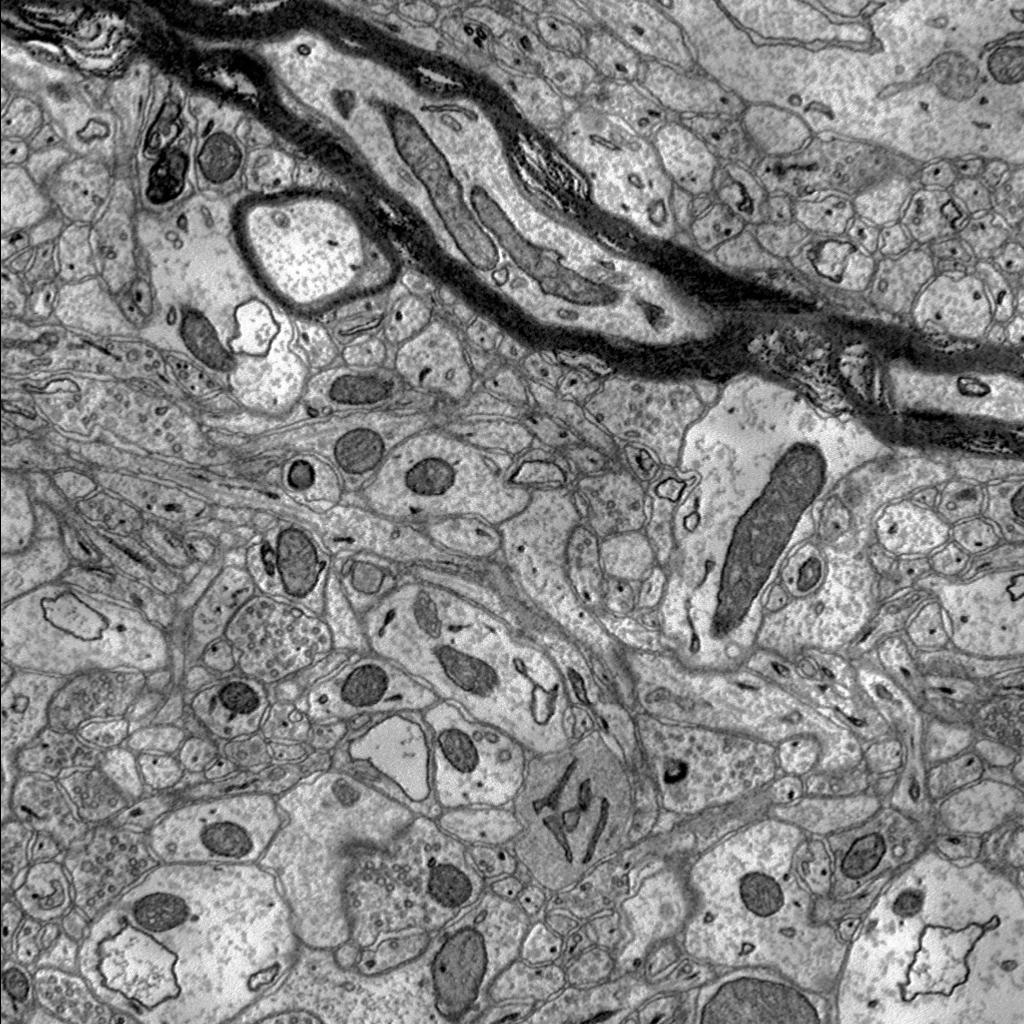
\includegraphics[width=0.22\linewidth]{./figures/pipeline/image.png}
	\hspace{0.025\linewidth}
	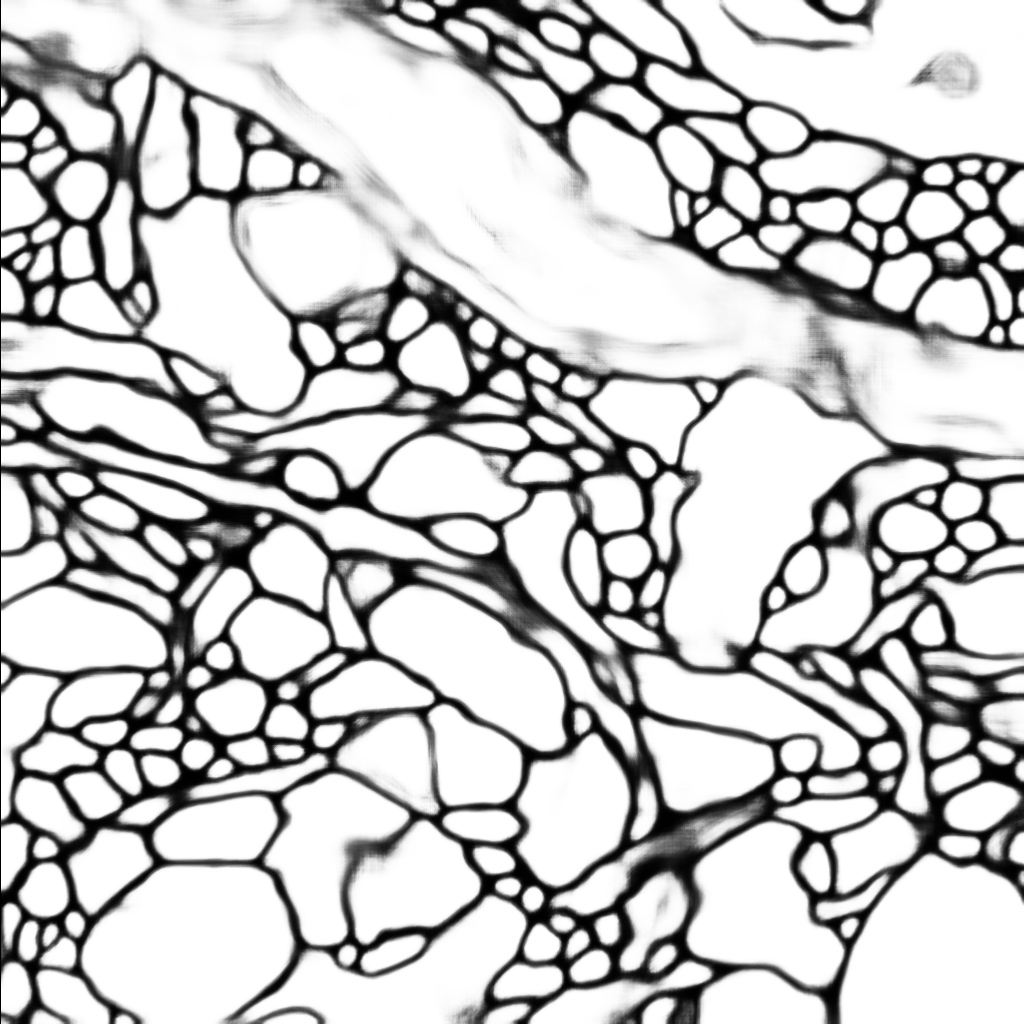
\includegraphics[width=0.22\linewidth]{./figures/pipeline/affinities.png}
	\hspace{0.025\linewidth}
	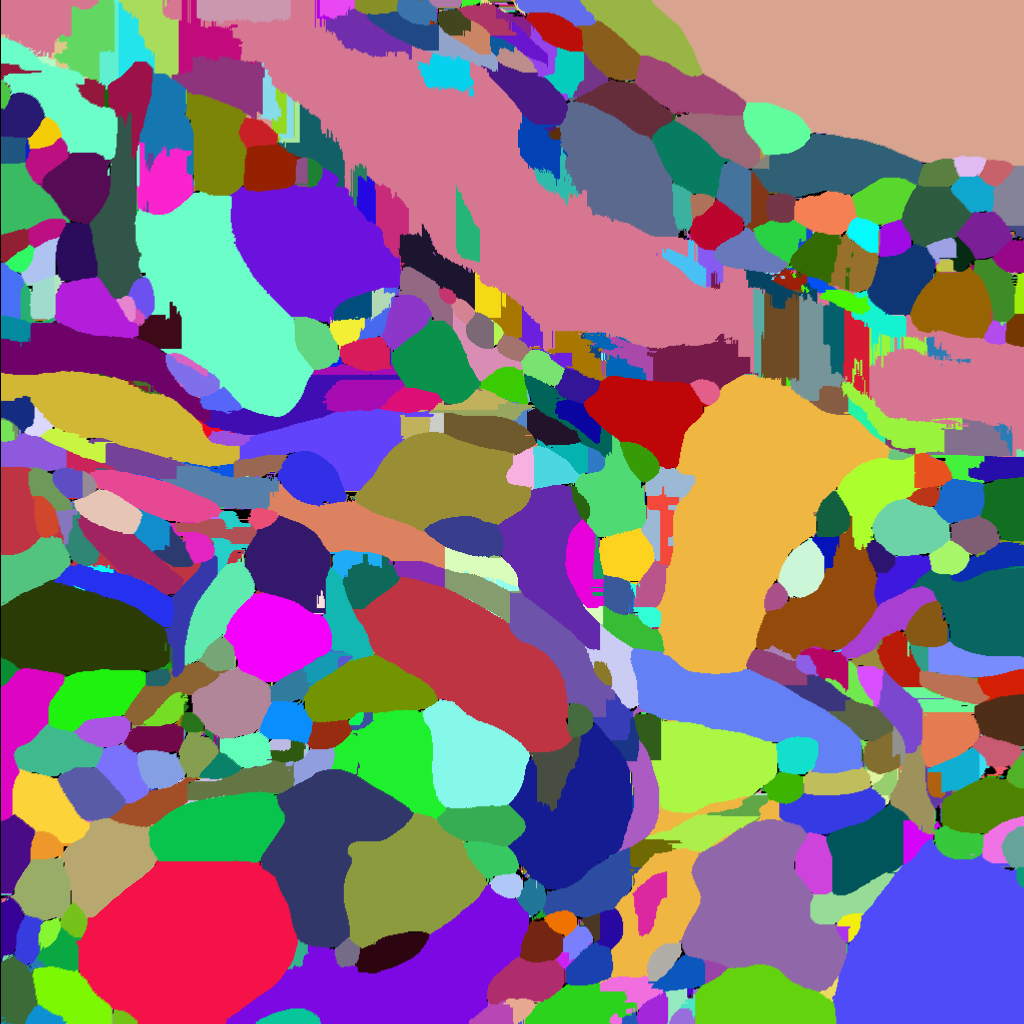
\includegraphics[width=0.22\linewidth]{./figures/pipeline/watershed.png}
	\hspace{0.025\linewidth}
	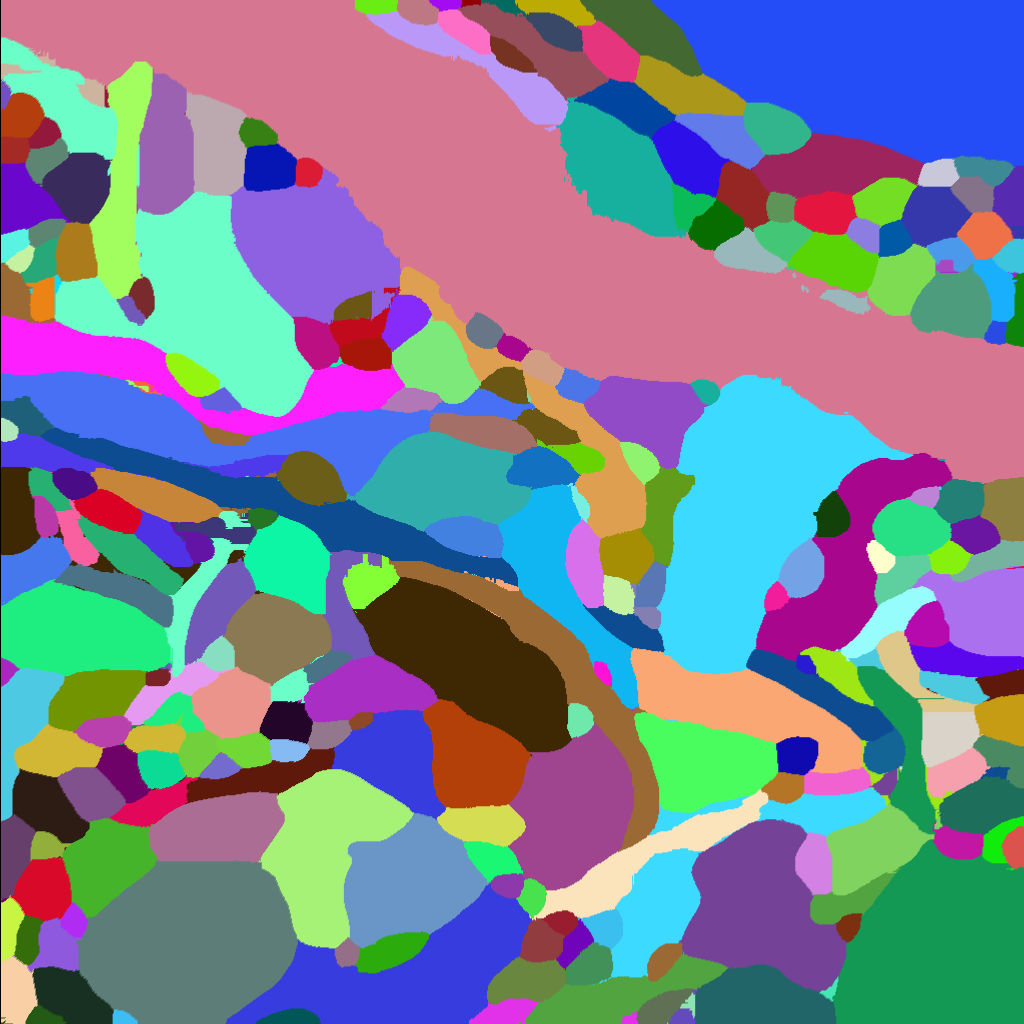
\includegraphics[width=0.22\linewidth]{./figures/pipeline/neuroproof.png}
	\caption{An overview of the existing methods. On the left is the original EM image data. A neural network (here VD2D3D) predicts the affinities between neighboring voxels. The Zwatershed algorithm clusters these voxels into supervoxels. NeuroProof agglomerates these supervoxels to create larger segments.}
	\label{fig:pipeline}
\end{figure*}

\paragraph{Voxel-based methods.} 
A large amount of connectomics research considers the problem of extracting segmentation information at the voxel level from the raw EM images to produce label volumes.
In a label volume, every voxels receives a segment label corresponding to a unique neuron.
Voxels with the same segment label belong to the same neuron. 
Such works focus on training 2-D convolutional neural networks to predict membrane probabilities per image slice~\cite{ciresan2012deep,jain2010boundary,amelio_segmentation,rhoananet,kaynig2015large}. 
More recent strategies augment these neural networks with the $z$-dimension creating full 3-D convolutional networks~\cite{lee2015recursive}.
Oftentimes these networks produce probabilities for the affinity between voxels rather than probabilities for a voxel belonging to a cell membrane~\cite{ronneberger2015u}. 
A sizable amount of computer vision research analyzes various hand-designed shape features for determining similarity between objects~\cite{osada2002shape} and for segmentation\cite{conners1984segmentation}. 
Currently, the random-forest classifiers used in connectomics rely on hand-designed features to make merge decisions.
Some of these features encode the distribution of probabilities that voxels along a segment boundary belong to the same neuron as their neighbors~\cite{nunez2014graph,ren2003learning}.
However, there is evidence that machine-learned features outperform hand-designed ones~\cite{bogovic2013learned}.
An extensive amount of research in computer vision, applied mathematics, and statistics evaluates the loss functions and optimizers for these networks~\cite{chatfield2014return,maas2013rectifier,nesterov1983method}. 

\paragraph{Super-voxel methods.} 
These approaches generate probabilities that neighboring voxels belong to the same neuron.
Many algorithms work at the resulting supervoxel level and train random-forest classifiers to produce segmentations of the EM images where every unique neuron in the volume has a unique label~\cite{seymour2016rhoananet,nunez2014graph,parag2017anisotropic,zlateski2015image} (CITE NEUROPROOF). 
Despite the success of these classifiers, they often make mistakes based on the local information leading to errors in the segmentation. 
Proofreading methods create a ``human-in-the-loop" framework that allows users to find errors and correct them \cite{haehn2017scalable,haehn2017guided,haehn2014design,error_correction_using_CNN}. 

More recently, flood-filling networks merge the process of generating voxel affinities and then producing segmentations by training an end-to-end neural network that outputs segmentations~\cite{januszewski2016flood}. 
These networks produce impressive segmentation accuracies of over $X\%$.%TODO ADD ACCURACY FOR FLOOD FILLING NETWORKS

\paragraph{Graph-based methods.} 
Many segmentation and clustering algorithms use graph partitioning techniques~\cite{andres2012globally} or normalized cuts for image segmentation~\cite{kappes2016higher,shi2000normalized,tatiraju2008image}. 
The multicut graph partitioning algorithm extracts segments the graph and remove edges such that there are no cycles. 
This closely resembles the biological constraint that neurons have a topological genus of zero. 
There are several useful multicut heuristics which provide good approximations with reasonable computational costs~\cite{horvnakova2017analysis,kernighan1970efficient,keuper2015efficient}

\paragraph{Skeletonization methods.} We use a graph-based abstraction of segmentation data based on skeletonizations. 
This topic is the focus of extensive research in the fields of computer graphics, mathematics, and biomedical visualization.
%The fields of computer graphics, mathematics, and biomedical visualization produce extensive research into the skeletonization of 3D binary volumes. 
Some of the research explores topologically consistent thinning algorithms and potential medical applications of these methods~\cite{palagyi20003d,palagyi2001sequential}. 
In computer graphics, fast medial axis algorithms allow animators to quickly move characters through successive frames~\cite{baran2007automatic,bharaj2012automatically}. 
In these works, the skeleton acts as the simplest representation of a 3-D volume. 
The Tree-structure Extraction Algorithm for Accurate and Robust Skeletons (TEASER) has been used by connectomics researchers to parameterize 3-D shapes~\cite{sato2000teasar,zhao2014automatic}. 
